\chapter{Materials and Methods}

\section{Materials}

\subsection{Simulation Enviornment}

\begin{itemize}
   \item \textbf{programming language:} Python 3.10
   \item \textbf{robotics simulator:} PyBullet 3.2.0
   \item \textbf{quadruped robot 3D model:} Unitree A1
   \item \textbf{packages that extend Python's array programming capability:}
      \subitem Numpy 1.22.2
      \subitem Pandas 1.4.0
\end{itemize}

\subsection{Development Environment}

\begin{itemize}
   \item \textbf{terminal emulator:} Windows Terminal
   \item \textbf{shell:} PowerShell 7.2.1
   \item \textbf{package manager:} Scoop
   \item \textbf{Python version manager:} pyenv-win
   \item \textbf{Python packaging and dependency manager:} Poetry
   \item \textbf{version control system:} Git
   \item \textbf{code hosting platform:} GitHub
   \item \textbf{languages for documentation:}
      \subitem Markdown
      \subitem \LaTeXe
         \subsubitem TeX distribution: MiKTeX 21.12
         \subsubitem typesetting engine: XeTeX
         \subsubitem reference management: BibTeX
      \subitem Mermaid 8.14.0
   \item \textbf{editor:} VSCode
      \subitem \textbf{Python support:} Python extension pack 2022.2.1924087327
      \subitem \textbf{Markdown support:} Markdown All in One 3.4.0
      \subitem \textbf{\LaTeX\ support:} LaTeX Workshop 8.23.0
   \item \textbf{3D CAD modeling:} Shapr3D
   \item \textbf{file format:} EditorConfig
   \item \textbf{blog framework:} Hexo
      \subitem \textbf{theme:} NexT
      \subitem \textbf{Markdown renderer:} hexo-renderer-marked
      \subitem \textbf{MathJax renderer:} hexo-filter-mathjax
   \item \textbf{static site hosting service:} GitHub Pages
\end{itemize}

\newpage
\section{Methods}

\subsection{Modelling}

Firstly, a geometric model of the quadruped robot was established.

\begin{figure}[htbp]
   \centering
   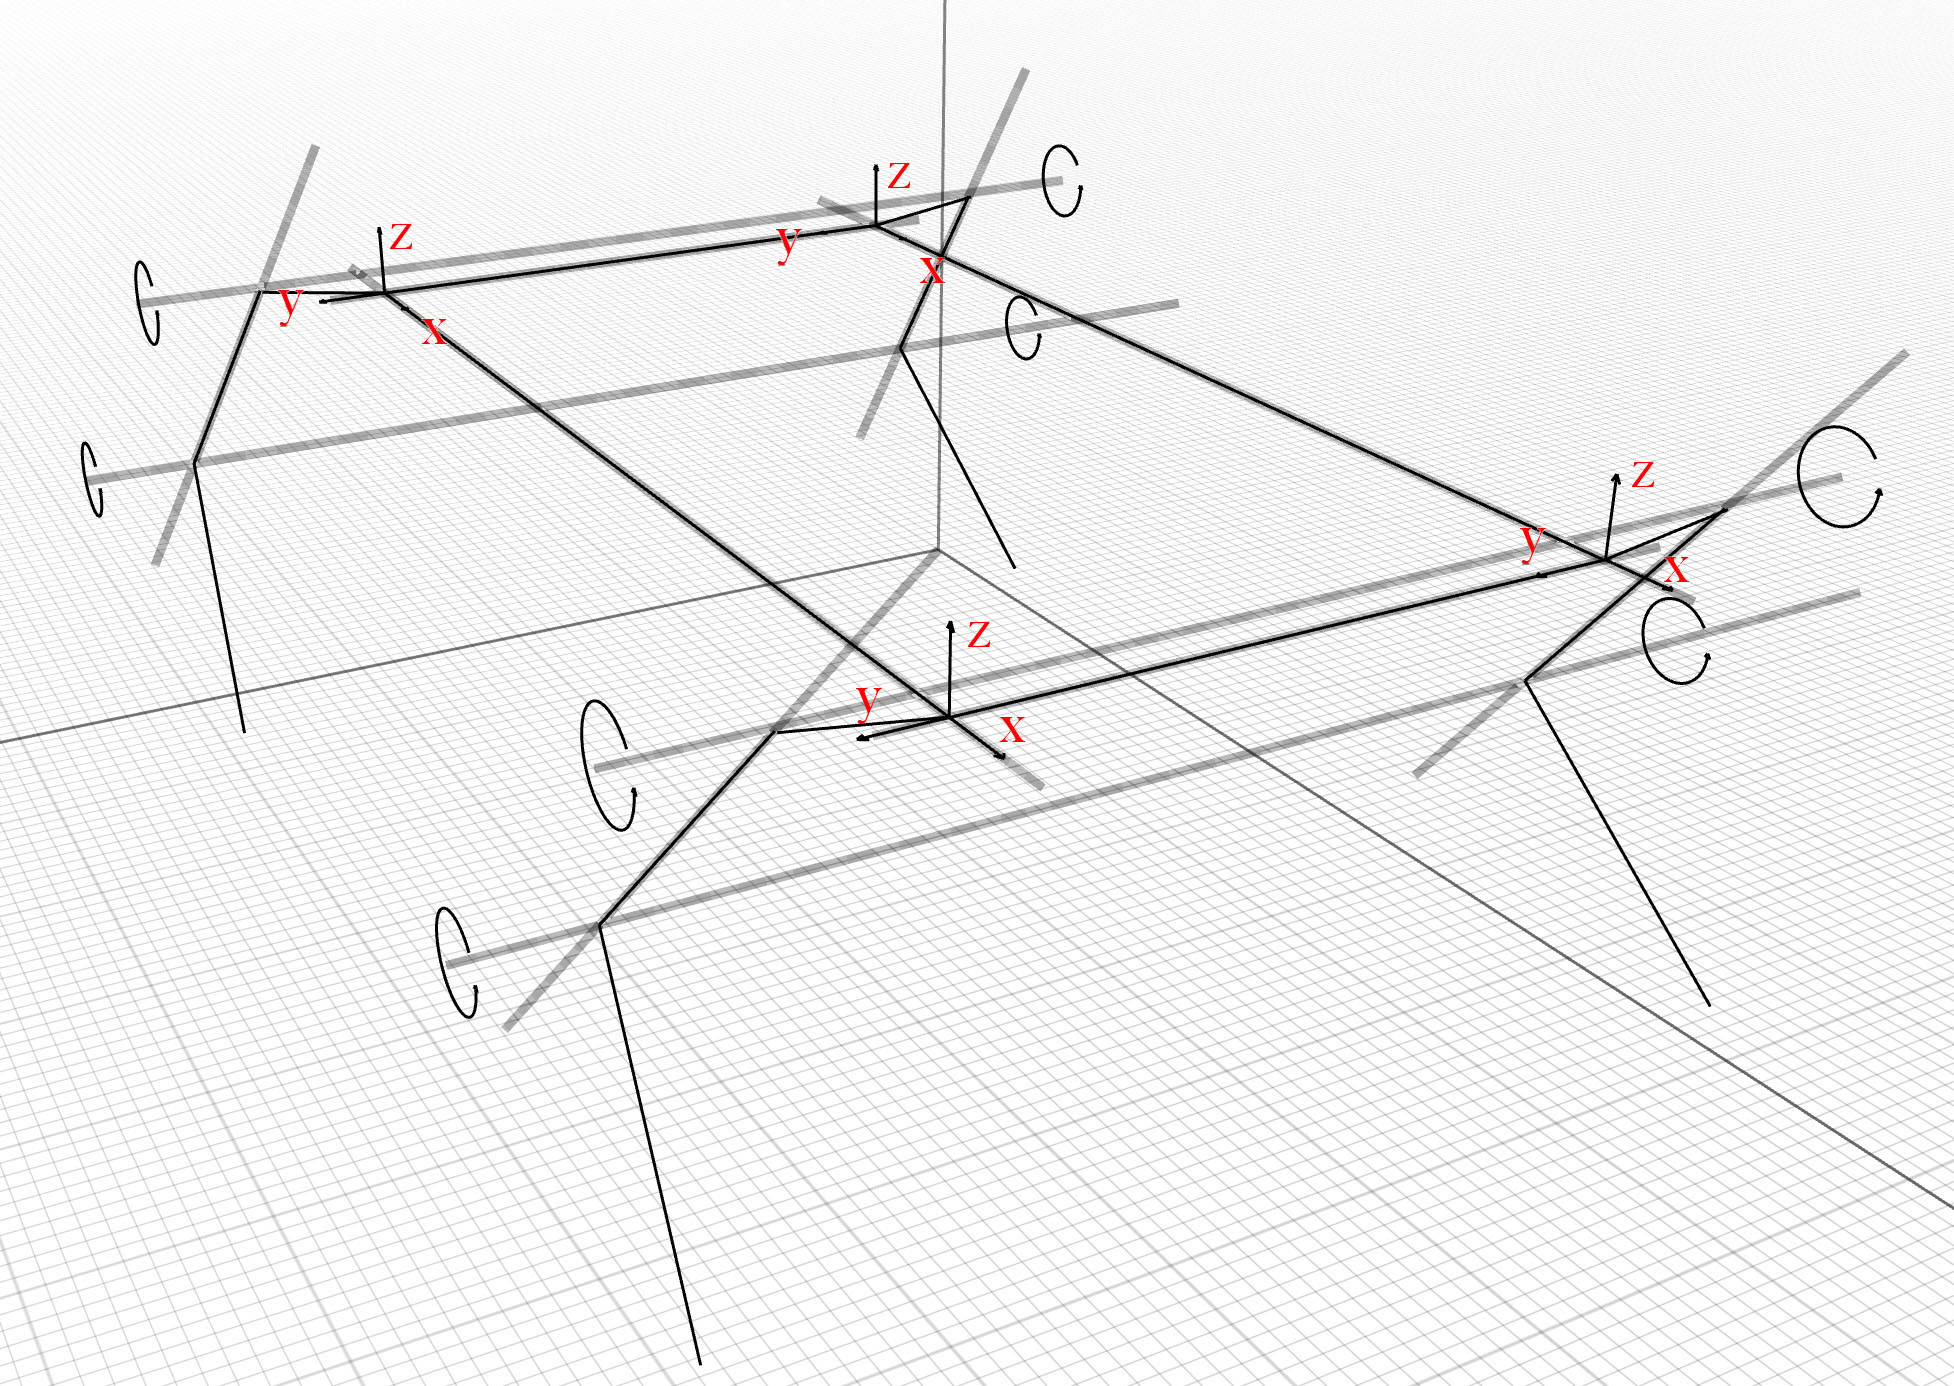
\includegraphics[width=0.65\textwidth]{figures/geometric_model.jpg}
   \caption{Geometric model of the quadruped robot}
   \label{fig:geometric_model}
\end{figure}

Figure \ref{fig:geometric_model} shows a trimetric view of the model. The body is reduced to a square and the legs are reduced to three connecting rods. The joint between the body and the legs is called hip. The uppermost rod of the leg is called the hip offset, followed by the thigh and finally the shank. In a robot entity, the distance from centre of motor controlling hip abduction/adduction to top centre of the thigh is approximated by the hip offset.

\begin{figure}[htbp]
   \centering
   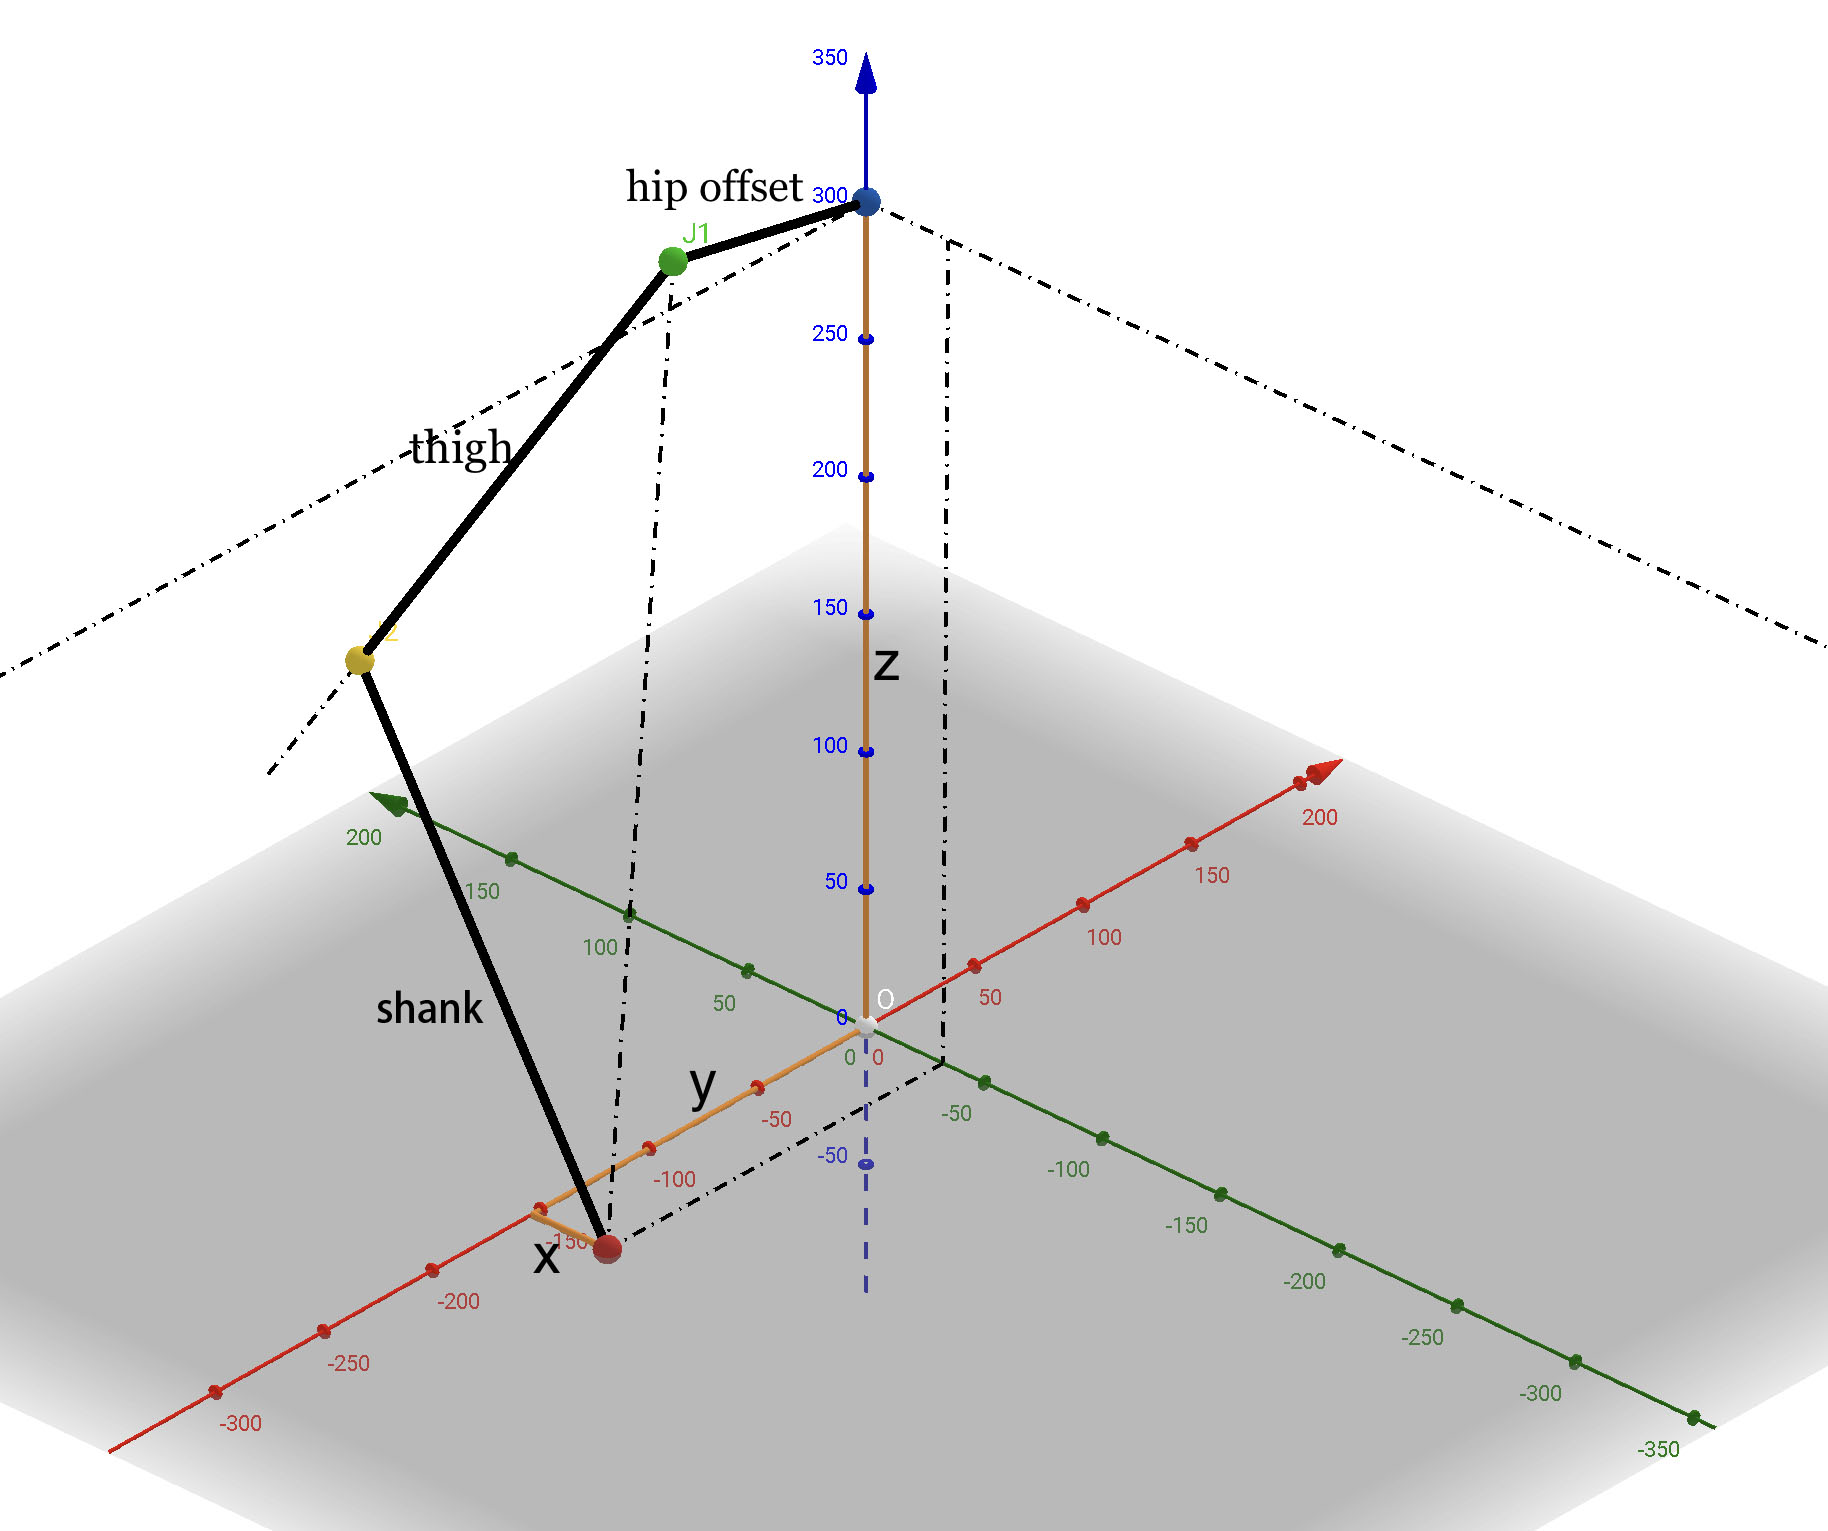
\includegraphics[width=0.7\textwidth]{figures/right_leg_model.jpg}
   \caption{Right leg model}
   \label{fig:right_leg_model}
\end{figure}

The leg has four important parts. There are three movable parts, named hip abduction/adduction (abd/add) joint, hip flextion/extension (fle/ext) joint, and knee joint from top to bottom. The end of the leg is called toe.

In order to describe leg movements using mathematics, it is first necessary to establish a coordinate system. In terms of leg movements, the hip and the toe are the parts of the leg that receive the most attention; because once the position of the toe in relation to the hip has been determined, the shape of the leg is fixed. The hip is located in the body and is a immovable point for the body, so setting it as the origin is convient for thinking. The positive direction of the coordinate system is shown in Figure \ref{fig:geometric_model}. There will be a coordinate system on each hip. This means that the four legs will be studied separately.

Specifying initial position of the motor and positive direction of rotation is as important as establishing the coordinate system. The quadruped robot model used for this project, Unitree A1, specifies them in its unified-robotics-description-format file, so these provisions are directly followed. The initial position of the motors and the positive direction of rotation is shown in Figure <++>.

% \begin{figure}[htbp]
%    \centering
%    \includegraphics[width=0.8\textwidth]{figures/}
%    \caption{}
%    \label{fig:}
% \end{figure}

The Unitree A1's unified-robotics-description-format file also specifies the boundary positions of the motors. They are listed in Table \ref{table:motors_boundary_positions}. For the sake of readability, front-left is abbreviated as fl, front-right as fr, hind-left as hl, and hind-right as hr.

\begin{table}[htbp]
   \centering
   \caption{Motors boundary positions}
   \begin{tabular}{|c|c|c|}
   \hline
   Motors & Positive Boundary (rad) & Negative Boundary (rad) \\ \hline
   fl hip abd/add &  0.803 & -0.803 \\ \hline
   fr hip abd/add &  0.803 & -0.803 \\ \hline
   hl hip abd/add &  0.803 & -0.803 \\ \hline
   hr hip abd/add &  0.803 & -0.803 \\ \hline
   fl hip fle/ext &  4.189 & -1.047 \\ \hline
   fr hip fle/ext &  4.189 & -1.047 \\ \hline
   hl hip fle/ext &  4.189 & -1.047 \\ \hline
   hr hip fle/ext &  4.189 & -1.047 \\ \hline
   fl knee        & -0.916 & -2.697 \\ \hline
   fr knee        & -0.916 & -2.697 \\ \hline
   hl knee        & -0.916 & -2.697 \\ \hline
   hr knee        & -0.916 & -2.697 \\ \hline
   \end{tabular}
   \label{table:motors_boundary_positions}
\end{table}

The next step is to derive the relationship between the toe coordinates before and after posture adjustment. The posture adjustment including pitching, yawing, rolling, and squatting.

\subsubsection{Pitching}

When pitching, the body length is constant, and the central axis of the body remains in the same position. Using these two conditions, the coordinates after pitching can be obtained by transforming the coordinate system three times. Take the front-right leg as an example:

\begin{figure}[htbp]
   \centering
   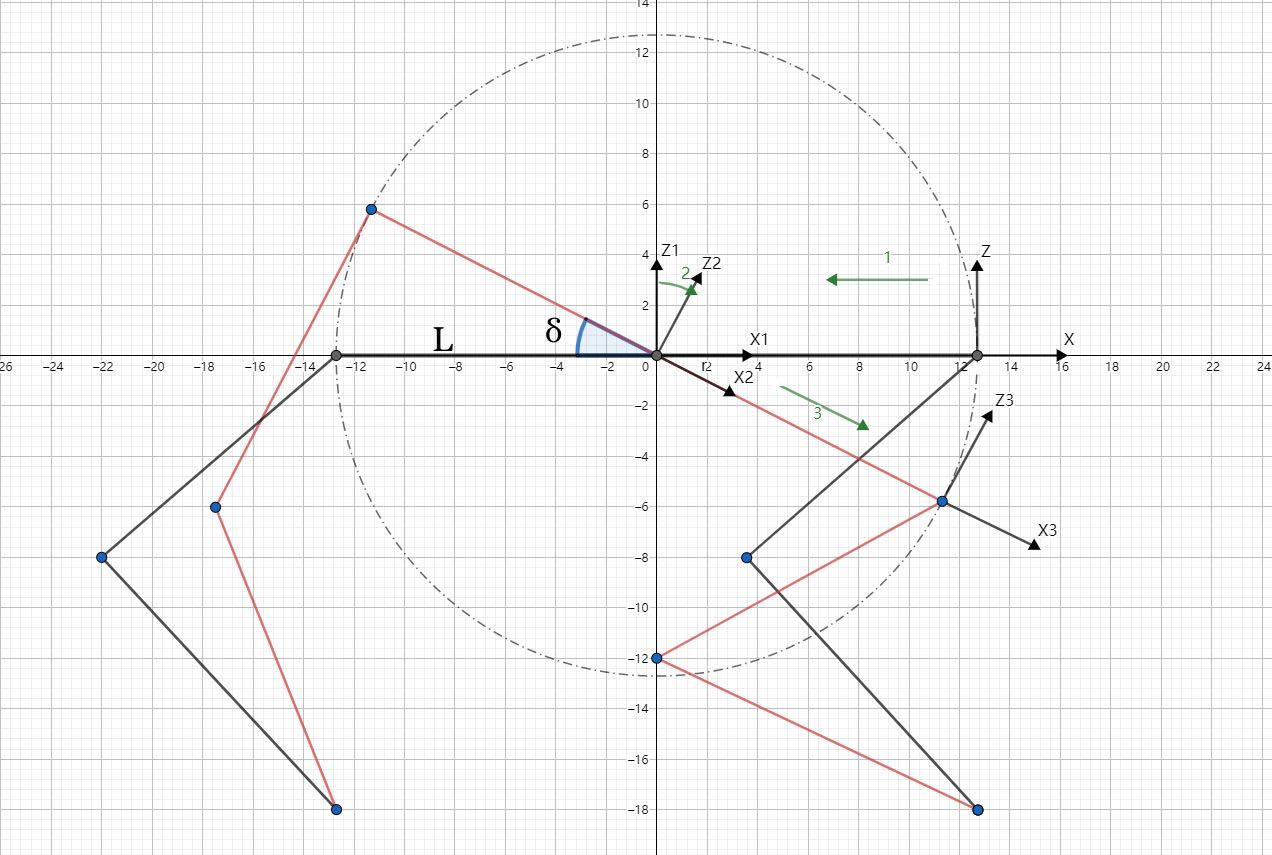
\includegraphics[width=0.8\textwidth]{figures/coordinate_transformations_in_pitching.jpg}
   \caption{Coordinate transformations in pitching}
   \label{fig:coordinate_transformations_in_pitching}
\end{figure}

The process of translating the coordinate system from hip to the central axis can be described by pre-multipling a transformation matrix:
\begin{equation}
   \begin{bmatrix}
   x_\text{after translating} \\
   z_\text{after translating} \\
   1                          \\
   \end{bmatrix}
   =
   \begin{bmatrix}
   1 & 0 & L \\
   0 & 1 & 0 \\
   0 & 0 & 1 \\
   \end{bmatrix}
   \begin{bmatrix}
   x \\
   z \\
   1 \\
   \end{bmatrix}
\end{equation}

where L is half body length.

Then, rotate the coordinate system by the pitching angle $\delta$ and transform it to the new location of the hip. The matrix multiplication for this process is
\begin{equation}
   \begin{bmatrix}
   x_\text{after pitching} \\
   z_\text{after pitching} \\
   1                       \\
   \end{bmatrix}
   =
   \begin{bmatrix}
   \cos\delta & -\sin\delta & -L \\
   \sin\delta & \cos\delta & 0 \\
   0 & 0 & 1 \\
   \end{bmatrix}
   \begin{bmatrix}
   x_\text{after translating} \\
   z_\text{after translating} \\
   1                          \\
   \end{bmatrix}
\end{equation}

The coordinates after pitching are obtained. Note that the y-coordinate does not change when pitching.

The two two matrix multiplication above can be combined into one
\begin{equation}\label{eq:pitching_fr_leg}
   \begin{bmatrix}
   x_\text{after pitching} \\
   z_\text{after pitching} \\
   1                       \\
   \end{bmatrix}
   =
   \begin{bmatrix}
   \cos\delta & -\sin\delta & L \times \cos\delta - L \\
   \sin\delta & \cos\delta & L \times \sin\delta \\
   0 & 0 & 1 \\
   \end{bmatrix}
   \begin{bmatrix}
   x \\
   z \\
   1 \\
   \end{bmatrix}
\end{equation}

The above calculation process is all for the front-right leg. By calculating the other legs it can be seen that for both \textbf{front} legs Eq \ref{eq:pitching_fr_leg} holds. For \textbf{hind} legs, the equation is
\begin{equation}
   \begin{bmatrix}
   x_\text{after pitching} \\
   z_\text{after pitching} \\
   1                       \\
   \end{bmatrix}
   =
   \begin{bmatrix}
   \cos\delta & -\sin\delta & -L \times \cos\delta + L \\
   \sin\delta & \cos\delta & -L \times \sin\delta \\
   0 & 0 & 1 \\
   \end{bmatrix}
   \begin{bmatrix}
   x \\
   z \\
   1 \\
   \end{bmatrix}
\end{equation}

Adding the information that y does not change during pitching to the matrix multiplication, the final form for the \textbf{front} legs is
\begin{equation}
   \begin{bmatrix}
   x_\text{after pitching} \\
   y_\text{after pitching} \\
   z_\text{after pitching} \\
   1                       \\
   \end{bmatrix}
   =
   \begin{bmatrix}
   \cos\delta & 0 & -\sin\delta & L \times \cos\delta - L \\
   0 & 1 & 0 & 0 \\
   \sin\delta & 0 & \cos\delta & L \times \sin\delta \\
   0 & 0 & 0 & 1 \\
   \end{bmatrix}
   \begin{bmatrix}
   x \\
   y \\
   z \\
   1 \\
   \end{bmatrix}
\end{equation}

and for the \textbf{hind} legs is
\begin{equation}
   \begin{bmatrix}
   x_\text{after pitching} \\
   y_\text{after pitching} \\
   z_\text{after pitching} \\
   1                       \\
   \end{bmatrix}
   =
   \begin{bmatrix}
   \cos\delta & 0 & -\sin\delta & -L \times \cos\delta + L \\
   0 & 1 & 0 & 0 \\
   \sin\delta & 0 & \cos\delta & -L \times \sin\delta \\
   0 & 0 & 0 & 1 \\
   \end{bmatrix}
   \begin{bmatrix}
   x \\
   y \\
   z \\
   1 \\
   \end{bmatrix}
\end{equation}

\subsubsection{Yawing}

The above idea also applies to yawing. One difference is that the matrix for translating each of the four coordinate systems is different, so that ultimately each leg corresponds to a matrix. See Figure \ref{fig:coordinate_transformations_in_yawing}.

\begin{figure}[htbp]
   \centering
   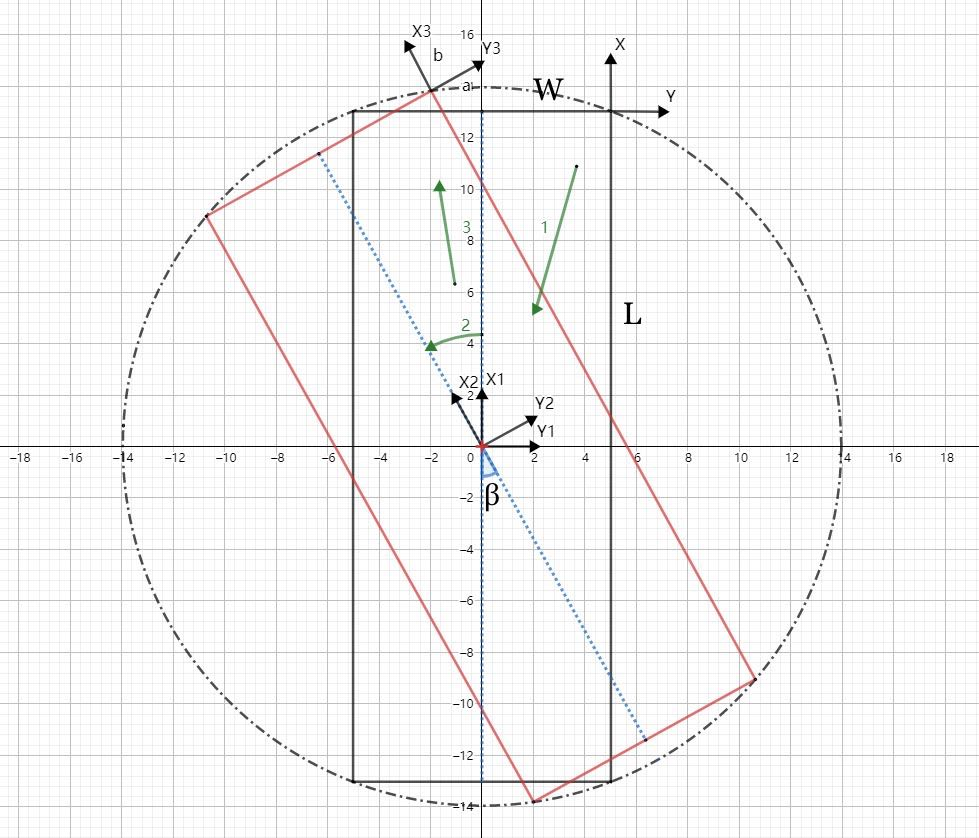
\includegraphics[width=0.8\textwidth]{figures/coordinate_transformations_in_yawing.jpg}
   \caption{Coordinate transformations in yawing}
   \label{fig:coordinate_transformations_in_yawing}
\end{figure}

As the derivation has already been described in section Pitching, it is omitted here, and the final form of matrix multiplication for yawing for each leg are listed directly. Give that the yawing angle is $\beta$, half body length is L, and half body width is W.

For \textbf{front-right} leg:
\begin{equation}
   \begin{bmatrix}
   x_\text{after yawing} \\
   y_\text{after yawing} \\
   z_\text{after yawing} \\
   1                     \\
   \end{bmatrix}
   =
   \begin{bmatrix}
   \cos\beta & -\sin\beta & 0 & L \times \cos\beta - W \times \sin\beta - L \\
   \sin\beta & \cos\beta & 0 & L \times \sin\beta + W \times \cos\beta - W \\
   0 & 0 & 1 & 0 \\
   0 & 0 & 0 & 1 \\
   \end{bmatrix}
   \begin{bmatrix}
   x \\
   y \\
   z \\
   1 \\
   \end{bmatrix}
\end{equation}

For \textbf{front-left} leg:
\begin{equation}
   \begin{bmatrix}
   x_\text{after yawing} \\
   y_\text{after yawing} \\
   z_\text{after yawing} \\
   1                     \\
   \end{bmatrix}
   =
   \begin{bmatrix}
   \cos\beta & -\sin\beta & 0 & L \times \cos\beta + W \times \sin\beta - L \\
   \sin\beta & \cos\beta & 0 & L \times \sin\beta - W \times \cos\beta + W \\
   0 & 0 & 1 & 0 \\
   0 & 0 & 0 & 1 \\
   \end{bmatrix}
   \begin{bmatrix}
   x \\
   y \\
   z \\
   1 \\
   \end{bmatrix}
\end{equation}

For \textbf{hind-right} leg:
\begin{equation}
   \begin{bmatrix}
   x_\text{after yawing} \\
   y_\text{after yawing} \\
   z_\text{after yawing} \\
   1                     \\
   \end{bmatrix}
   =
   \begin{bmatrix}
   \cos\beta & -\sin\beta & 0 & -L \times \cos\beta - W \times \sin\beta + L \\
   \sin\beta & \cos\beta & 0 & -L \times \sin\beta + W \times \cos\beta - W \\
   0 & 0 & 1 & 0 \\
   0 & 0 & 0 & 1 \\
   \end{bmatrix}
   \begin{bmatrix}
   x \\
   y \\
   z \\
   1 \\
   \end{bmatrix}
\end{equation}

For \textbf{hind-left} leg:
\begin{equation}
   \begin{bmatrix}
   x_\text{after yawing} \\
   y_\text{after yawing} \\
   z_\text{after yawing} \\
   1                     \\
   \end{bmatrix}
   =
   \begin{bmatrix}
   \cos\beta & -\sin\beta & 0 & -L \times \cos\beta + W \times \sin\beta + L \\
   \sin\beta & \cos\beta & 0 & -L \times \sin\beta - W \times \cos\beta + W \\
   0 & 0 & 1 & 0 \\
   0 & 0 & 0 & 1 \\
   \end{bmatrix}
   \begin{bmatrix}
   x \\
   y \\
   z \\
   1 \\
   \end{bmatrix}
\end{equation}

\subsubsection{Rolling}

Unlike yawing, in rolloing, the right two legs share a transformation matrix, as do the left two legs. This is because the translation operation of the coordinate system is different for the left and right sides, while the rotation operation is the same for each leg.

\begin{figure}[htbp]
   \centering
   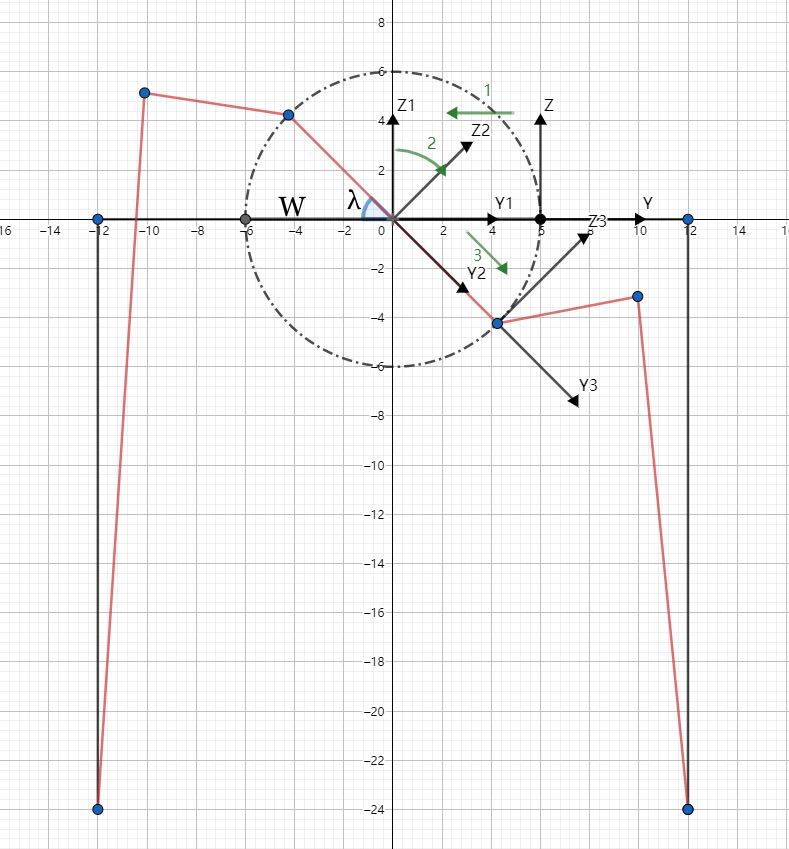
\includegraphics[width=0.6\textwidth]{figures/coordinate_transformations_in_rolling.jpg}
   \caption{Coordinate transformations in rolling}
   \label{fig:coordinate_transformations_in_rolling}
\end{figure}

Give that rolling angle is $\lambda$, and half body width is W. Again, the derivation is omitted and only the final form of matrix multiplication is presented.

For \textbf{right} legs:
\begin{equation}
   \begin{bmatrix}
   x_\text{after rolling} \\
   y_\text{after rolling} \\
   z_\text{after rolling} \\
   1                      \\
   \end{bmatrix}
   =
   \begin{bmatrix}
   1 & 0 & 0 & 0 \\
   0 & \cos\lambda & -\sin\lambda & W \times \cos\lambda - W \\
   0 & \sin\lambda & \cos\lambda & W \times \sin\lambda \\
   0 & 0 & 0 & 1 \\
   \end{bmatrix}
   \begin{bmatrix}
   x \\
   y \\
   z \\
   1 \\
   \end{bmatrix}
\end{equation}

For \textbf{left} legs:
\begin{equation}
   \begin{bmatrix}
   x_\text{after rolling} \\
   y_\text{after rolling} \\
   z_\text{after rolling} \\
   1                      \\
   \end{bmatrix}
   =
   \begin{bmatrix}
   1 & 0 & 0 & 0 \\
   0 & \cos\lambda & -\sin\lambda & -W \times \cos\lambda + W \\
   0 & \sin\lambda & \cos\lambda & -W \times \sin\lambda \\
   0 & 0 & 0 & 1 \\
   \end{bmatrix}
   \begin{bmatrix}
   x \\
   y \\
   z \\
   1 \\
   \end{bmatrix}
\end{equation}

\subsubsection{Squatting}

Squatting is actually the process of continuously changing the height of each hip above the ground. In all cases, the z-coordinate represents this height. Assuming that the standing surface does not change, then simply changing the z-coordinate can achieve a squat.

\subsection{Forward and Inverse Kinematics}

In the previous section, the transformation matrix of the coordinates of the toe after posture adjustment was obtained. However, only the motor position can be directly controlled, and also the robot's controller can only return information about the motor position and not the coordinates of the toe relative to the hip joint. Therefore, in order to control the motor position to achieve posture adjustment, both forward and inverse kinematics are required.

The forward kinematics means finding the coordinates of toe relative to the hip given motors position which is servo angle, while inverse kinematics is the opposite. This conversion relation can be derived elegantly using several mathematical concepts such as Euler angle. However, as it is too far beyond the knowledge of the team, the choice here is to use basic geometric knowledge to describe this relationship.

It is necessary to discuss the left and right sides in separate cases, as the Unitree A1's right-side motor configuration of the hip abd/add joint which includes initial position and positive direction does not consistent with the left side. Again, to save space, the equations on both sides are given directly.

\begin{figure}[htbp]
   \centering
   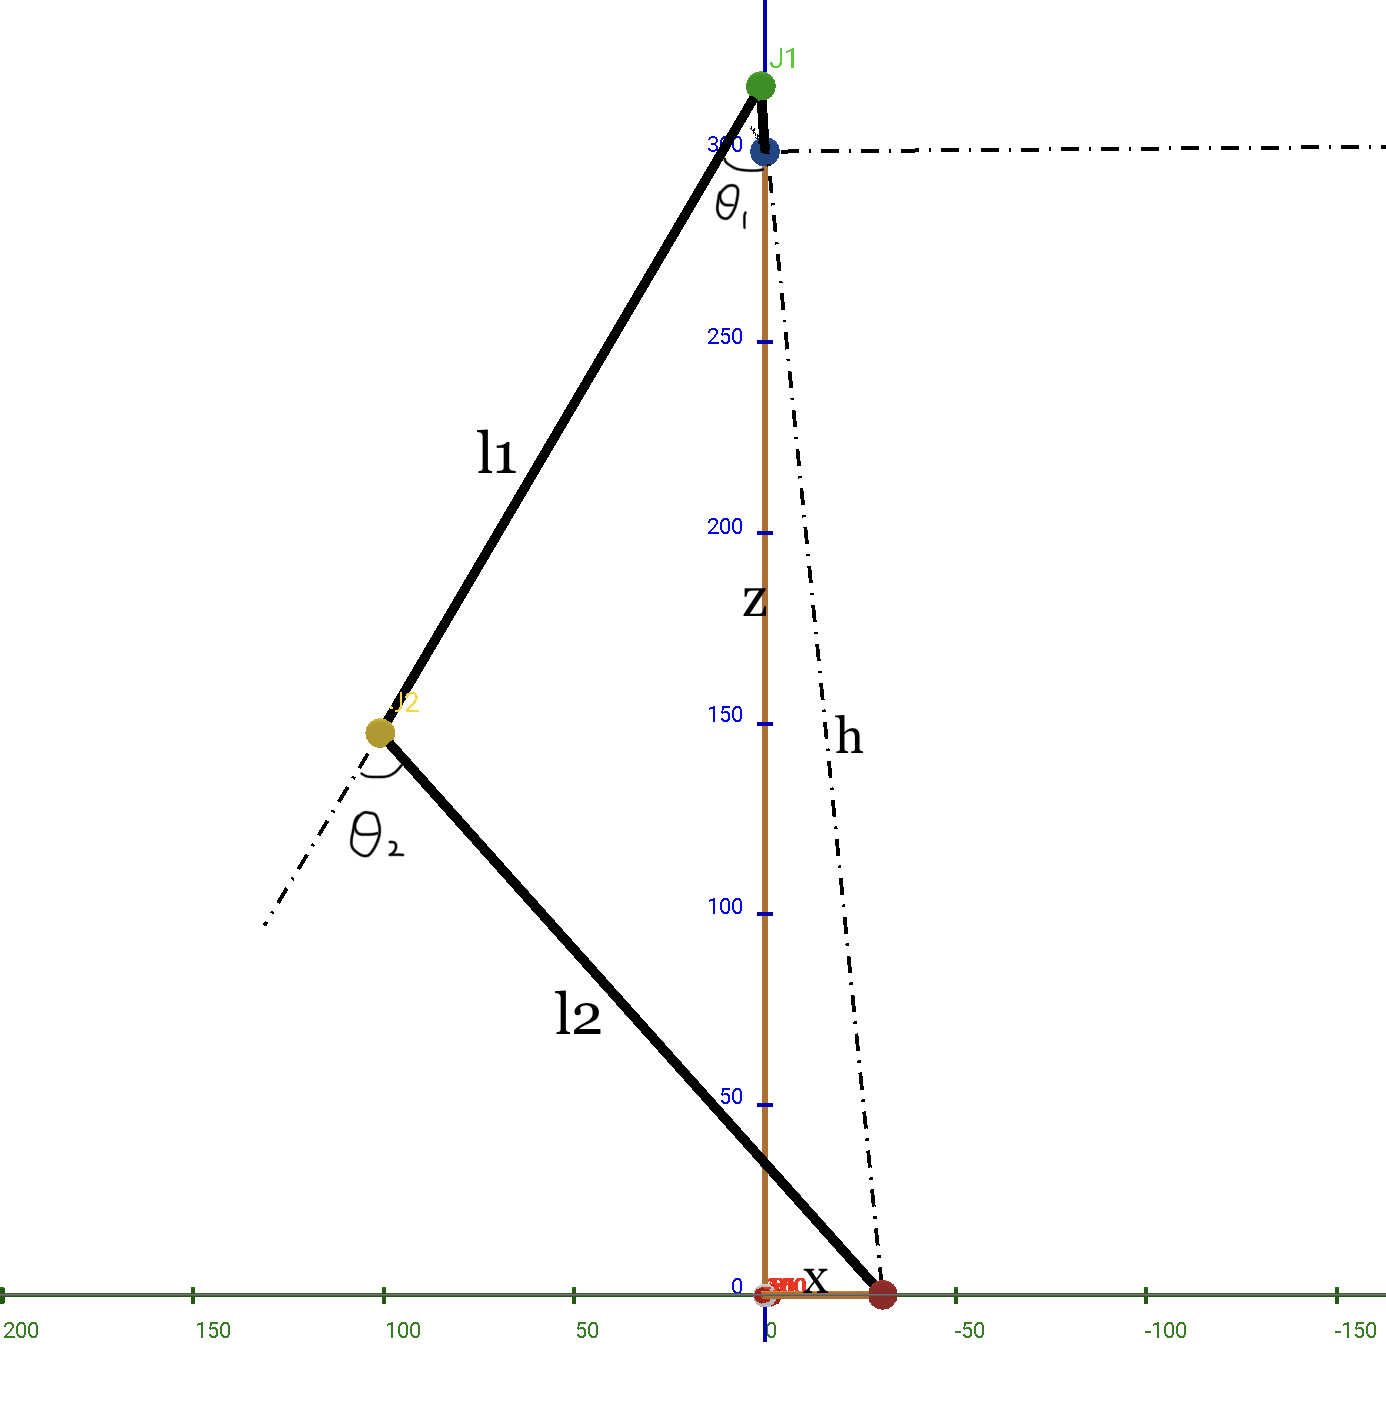
\includegraphics[width=0.58\textwidth]{figures/right_leg_model_left-side_view.jpg}
   \caption{Left-side view of the right leg model}
   \label{fig:right_leg_model_left-side_view}
\end{figure}

Give that thigh length is $l_1$, shank length is $l_2$, distance from the toe to the top point of the thigh rod is h, position of the hip fle/ext joint is $\theta_1$, and position of the knee joint is $\theta_2$. The following equation can be obtained easily from the left-side view of the right leg model shown in Figure \ref{fig:right_leg_model_left-side_view}.

$\theta_1, \theta_2 \rightarrow x, h$:
\begin{align*}
x &= -l_1 \times \sin\theta_1 - l_2 \times \sin(\theta_1 + \theta_2) \\
h &=  l_1 \times \cos\theta_1 + l_2 \times \cos(\theta_1 + \theta_2)
\end{align*}

$x, h \rightarrow \theta_1, \theta_2$:
\begin{align*}
\cos\theta_2 &= \frac{-l_1^2 - l_2^2 + x^2 + h^2}{2 l_1 l_2} \\
\sin\theta_2 &= -\sqrt{1 - \cos^2\theta_2} \\
\theta_1 &= \arccos(\frac{l_1^2 + x^2 + h^2 - l_2^2}{2 l_1 \sqrt{x^2 + h^2}}) - \arctantwo(\frac{x}{h}) \\
\theta_2 &= \arctantwo(\frac{\sin\theta_2}{\cos\theta_2})
\end{align*}

Give that the hip offset is o and position of hip abd/add joint is $\theta_3$. A second set of equations can be obtained from the front view of the right leg model (Figure \ref{fig:right_leg_model_front_view}). As mentioned above, the motor configuration of hip abd/add joint is different on the left and right side; hence, two sets of equations are required.

\begin{figure}[htbp]
   \centering
   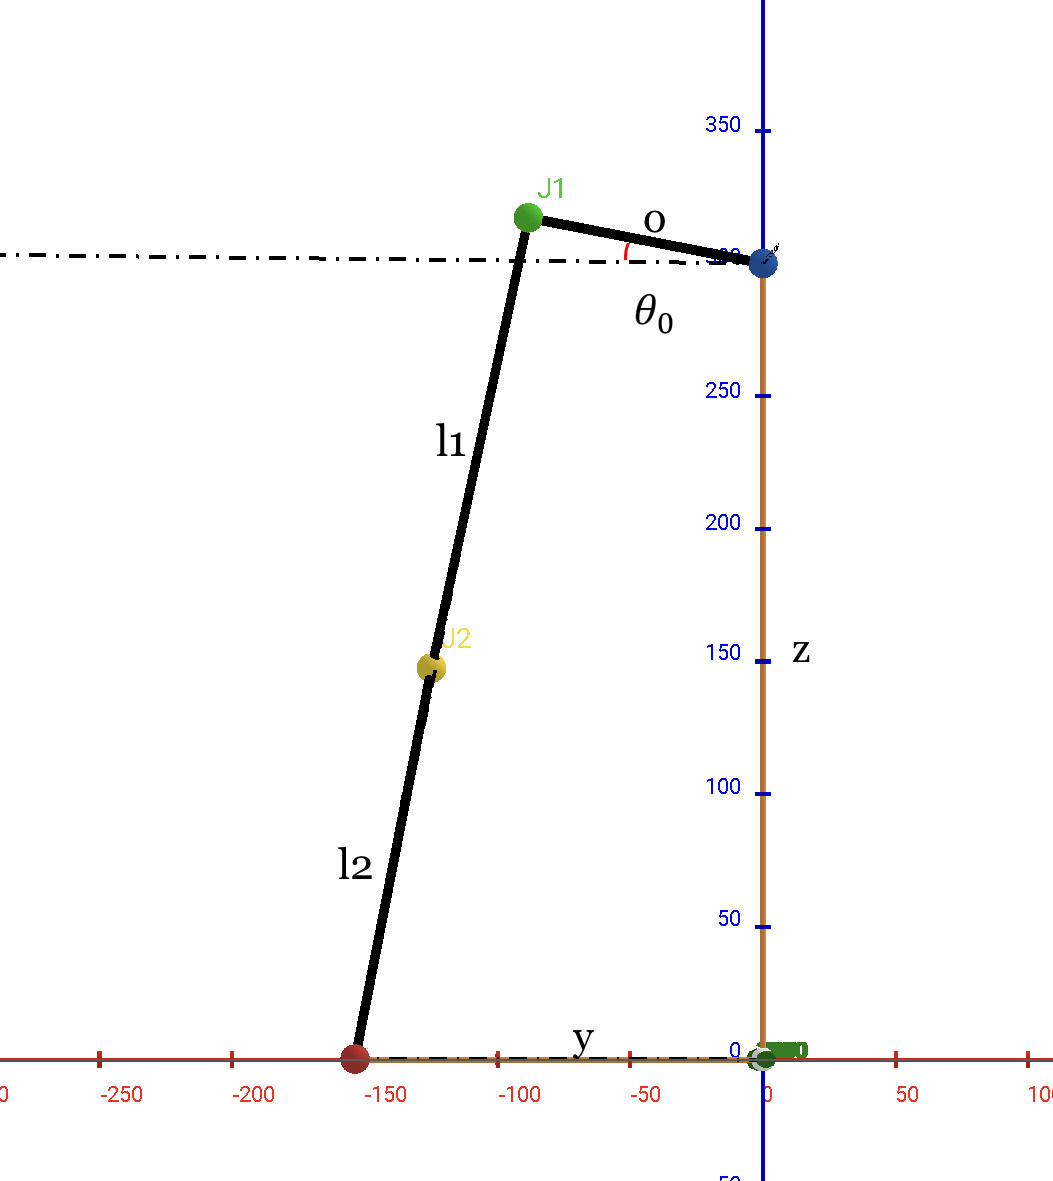
\includegraphics[width=0.55\textwidth]{figures/right_leg_model_front_view.jpg}
   \caption{Front view of the right leg model}
   \label{fig:right_leg_model_front_view}
\end{figure}

For the \textbf{right} side:

\indent\indent
$\theta_0 \rightarrow y, z$:
\begin{align*}
y &=  o \times \cos\theta_0 - h \times \sin\theta_0 \\
z &= -o \times \sin\theta_0 - h \times \cos\theta_0
\end{align*}

\indent\indent
$y, z \rightarrow \theta_0$:
\begin{equation*}
   \theta_0 = \arctantwo(\frac{\lvert z \lvert}{y}) - \arctantwo(\frac{h}{o})
\end{equation*}

but for the \textbf{left} side:

\indent\indent
$\theta_0 \rightarrow y, z$:
\begin{align*}
y &= -o \times \cos\theta_0 - h \times \sin\theta_0 \\
z &=  o \times \sin\theta_0 - h \times \cos\theta_0
\end{align*}

\indent\indent
$y, z \rightarrow \theta_0$:
\begin{equation*}
   \theta_0 = \arctantwo(\frac{h}{o}) - \arctantwo(\frac{\lvert z \lvert}{-y})
\end{equation*}

\subsubsection{Summary}

\noindent
Forward kinematics:

$\theta_1, \theta_2 \rightarrow x, h$:
\begin{align}
x &= -l_1 \times \sin\theta_1 - l_2 \times \sin(\theta_1 + \theta_2) \\
h &=  l_1 \times \cos\theta_1 + l_2 \times \cos(\theta_1 + \theta_2)
\end{align}

$\theta_0 \rightarrow y, z$ for \textbf{right} side:
\begin{align}
y &=  o \times \cos\theta_0 - h \times \sin\theta_0 \\
z &= -o \times \sin\theta_0 - h \times \cos\theta_0
\end{align}

$\theta_0 \rightarrow y, z$ for \textbf{left} side:
\begin{align}
y &= -o \times \cos\theta_0 - h \times \sin\theta_0 \\
z &=  o \times \sin\theta_0 - h \times \cos\theta_0
\end{align}

\noindent
Inverse kinematics:

$x, h \rightarrow \theta_1, \theta_2$:
\begin{align}
\cos\theta_2 &= \frac{-l_1^2 - l_2^2 + x^2 + h^2}{2 l_1 l_2} \\
\sin\theta_2 &= -\sqrt{1 - \cos^2\theta_2} \\
\theta_1 &= \arccos(\frac{l_1^2 + x^2 + h^2 - l_2^2}{2 l_1 \sqrt{x^2 + h^2}}) - \arctantwo(\frac{x}{h}) \\
\theta_2 &= \arctantwo(\frac{\sin\theta_2}{\cos\theta_2})
\end{align}

$y, z \rightarrow \theta_0$ for \textbf{right} side:
\begin{equation}
   \theta_0 = \arctantwo(\frac{\lvert z \lvert}{y}) - \arctantwo(\frac{h}{o})
\end{equation}

$y, z \rightarrow \theta_0$ for \textbf{left} side:
\begin{equation}
   \theta_0 = \arctantwo(\frac{h}{o}) - \arctantwo(\frac{\lvert z \lvert}{-y})
\end{equation}

\subsection{Coding}

Equation derivation and coding were carried out simultaneously. After a set of equations for a movement had been derived, a simple Python script was used to verify correctness. If the result seen in the simulator was correct, the algorithm in the script would then be encapsulated into a library.

Once a movement had been ecapsulated, a corresponding application was written for debugging and testing purpose. After all the movements completed, a demo application was written which used in presentation of bench inspection.
